% \'Equations différentielles et systèmes dynamiques en temps continu. Existence, unicité des solutions. Recherche des équilibres et linéarisation. Classification des équilibres en dimensions 1 et 2.

\progres{
  Rappel cours 4 :
  \begin{itemize}
    \item Différentiabilité, matrice jacobienne, composition
    \item Intégration et changement de variable
    \item Caractérisation des extremums
    \item Exercice à faire : extrema de $f(x, y) = x^3 + y^3 - 3xy$.
  \end{itemize}
  Programme cours 5 :
  \begin{itemize}
    \item Chapitre 3 : équations différentielles et systèmes dynamiques
    \item EDO en dimension 1 : solution maximale, stabilité
    \item EDO en dimension $n$ : cas linéaire
    \item EDO en dimension $n$ : cas non linéaire
  \end{itemize}
}

%-------------------------------------------------------------------------------
\paragraph*{Objectif.} 
On s'intéresse à une fonction 
$$
\begin{array}{rrcl}
  y : & \Rbb & \mapsto & \Rbb^n \\
  & t & \to & y(t) = [y_1(t) \dots y_n(t)]^\top 
\end{array}
$$
qui soit solution d'une équation {\em fonctionnelle} de la forme
$$
\nabla y(t) = F(y(t))
$$
où $F$ est une fonction de $\Rbb^n$ dans $\Rbb^n$. Une telle équation est appelée {\em équation différentielle ordinaire} (EDO, alias {\em ODE} en anglais).

Comme la notation le laisse entendre, la variable $t$ décrit typiquement un temps et $y(t)$ l'évolution d'un système à $n$ coordonnées au cours du temps partant d'une {\em condition initiale}
$$
y(t_0) = y_0.
$$
En notant $\dot y$ la dérivée de $y$ par rapport au temps, un tel {\em système dynamique} s'écrit donc
$$
\left\{\begin{array}{rcl}
        y(t_0) & = & y_0, \\
        \dot y & = & F(y).
       \end{array}\right.
$$

%-------------------------------------------------------------------------------
\paragraph*{Deux modèles classiques.}
\begin{description}
 \item[Lotka-Volterra:] $y(t) = [N(t) \; P(t)]^\top$ avec $N(t) =$ nombre de proies au temps $t$, $(t) = $ nombre prédateurs au temps $t$:
 $$
 \left\{ \begin{array}{rcl} 
  \dot N & = & r N - c N P \\
  \dot P & = & b N P  - m P
 \end{array} \right.
 $$
 \item[SIR :] $y(t) = [S(t) \; I(t) \; R(t)]^\top$ avec $S(t) =$ nombre de susceptibles au temps $t$, $I(t) =$ nombre d'infectés et $R(t) =$ nombre de 'remis' ({\em recovered}) :
 $$
 \left\{ \begin{array}{rcl} 
  \dot S & = & - r S I \\
  \dot I & = & r S I - a I \\
  \dot R & = & a I \\
 \end{array} \right.
 $$
 Un tel modèle est dit à compartiments, les compartiments étant les populations d'effectifs respectifs $S$, $I$ et $R$. 
\end{description}

Ces deux modèles sont fondés sur des sytèmes d'équations différentielles en dimension plus grande que 1 et non linéaires.

%-------------------------------------------------------------------------------
%-------------------------------------------------------------------------------
\section{Exemple en 1D et solution maximale, stabilité} \label{sec:EquaDiff-1DsolMaximale}
%-------------------------------------------------------------------------------

%-------------------------------------------------------------------------------
\paragraph*{ODE linéaire en dimension 1 : modèle de Malthus.}
L'EDO la plus simple en dimension 1 est l'équation linéaire
$$
\dot y = r y
$$
dont la solution est connue : 
$$
y(t) = a_0 e^{rt}.
$$
Le paramètre $a_0$ est alors déterminé par une condition 'initiale' : en imposant que $y(t_0) = y_0$, il vient
$$
a_0 = y_0 e^{-t_0} 
\qquad \Rightarrow \qquad
y(t) = y_0 e^{r(t-t_0)}.
$$
Ce modèle est connu en dynamique des population sous le nom de {\em modèle de Malthus} : il suppose que l'accroissement de la population est directement proportionnel à sa taille. Ce modèle n'inclue pas de limitation de la taille de la population et en prévoit donc une croissance indéfini pour $r > 0$ (et une extinction pour $r < 0$).


%-------------------------------------------------------------------------------
\subsection{Solution maximale} 
%-------------------------------------------------------------------------------

\begin{definition}[Solution du problème de Cauchy]
  Soit $F : \Rbb^n \mapsto \Rbb^n$, $I$ un ouvert de $\Rbb$, $t_0 \in I$ et $y_0 \in \Rbb$. La fonction $f : I \mapsto \Rbb^n$ est dite solution du \emph{problème de Cauchy}, 
  $$
  \left\{\begin{array}{rcl}
          y(t_0) & = & y_0, \\
          \dot y & = & F(y).
        \end{array}\right.
  $$
  sur $I$ si $f(t_0) = y_0$ et $\forall t \in I: \dot f(t) = F(f(t))$.
\end{definition}

\begin{theorem}[Cauchy-Lipschitz]
  Si $F$ est $C^1$ par morceaux, il existe une unique solution $f$ sur $I$ au problème de Cauchy qui soit maximale au sens où si $g$ est également solution sur $J$, alors $J \subset I$ et $g(t) = f(t)$ pour tout $t \in J$. $f$ est appelée solution maximale et $I$ intervalle maximal.
\end{theorem}

\remark
$f(t) = y_0 e^{r(t-t_0)}$ est donc l'unique solution du problème $\{y_0 = y(t_0), \; \dot y = r y\}$ sur l'intervalle maximal $\Rbb$.

%-------------------------------------------------------------------------------
\exemple{
  Pour déterminer la solution et l'intervalle maximal du problème
  $$
  \{y(0) = 1, \; \dot y = -c y^2\},
  $$
  on remarque que
  \begin{align*}
    \dot y & = -c y^2 & 
    & \Leftrightarrow & 
    c & = - \frac{\dot y}{y^2} = \frac{\partial}{\partial t} \frac1y \\
    \text{donc} \qquad 
    \frac1y & = a + ct & 
    & \Leftrightarrow &
    y(t) & = \frac1{a + ct} \qquad \text{pour } t \neq -\frac{a}c.
  \end{align*}
  La condition $y(0) = 1$ impose alors que $a = 1$, soit 
  $$
  f(t) = (1+ ct)^{-1}
  $$ 
  est donc solution maximale sur l'intervalle (maximal) $\Rbb \setminus \{-1/c\}$.
}

%-------------------------------------------------------------------------------
\subsection{Point d'équilibre, stabilité} 
%-------------------------------------------------------------------------------

\begin{definition}[Point d'équilibre]
  $y^* \ \Rbb^n$ est un point d'équilibre de l'ODE $\dot y = F(y)$ si $F(y^*) = 0$.
\end{definition}

\begin{definition}[Stabilité ($n = 1$)]
  Pour $n = 1$, un équilibre $y^*$ est dit (asymptotiquement) stable si il existe $\varepsilon > 0$ tel que pour tout $y_0 \in (y^* - \varepsilon, y^* + \varepsilon)$, la condition initiale $y(0) = y_0$ implique que 
  $$
  \lim_{t \to \infty} y(t) = y^*.
  $$
  Dans le cas contraire, il est dit {\em instable}. Le caractère stable ou instable d'un équilibre définit sa {\em nature}.
\end{definition}

\remark
Un équilibre est donc stable si toute (petite) perturbation $\varepsilon$ autour de $y^*$ laisse le système retourner dans l'état $y^*$.


%-------------------------------------------------------------------------------
\paragraph*{Modèle de Verhulst.}
Une façon simple d'empêcher la croissance indéfinie de la population prédite par le modèle de Malthus consiste à supposer que le taux de reproduction $\dot y / y$ décroît linéairement avec la taille de la population : 
\begin{equation} \label{eq:verhulst}
\dot y / y = r - cy
\qquad \Leftrightarrow \qquad
\dot y = y(r - cy).
\end{equation}
Ce modèle est connu sous le nom de {\em modèle de Verhulst}. On suppose que les paramètres $r$ et $c$ sont positifs et on ôse la condition initiale
$$
y(0) = y_0.
$$
\begin{description}
  \item[Points d'équilibre:] $y^* = 0$ et $y^* = K := r/c$ sont des points d'équilibre car alors $\dot y = F(y^*) = 0$.
  \item[Solution pour $y_0 \in \{0, K\}$:] la fonction $y(t)$ reste constante (car $\dot y(t) \equiv 0$).
  \item[Solution pour $0 < y_0 < K$:]  
  On obtient une solution de cette équation en remarquant que, pour $t$ tel que $0 < y(t) < K$, \eqref{eq:verhulst} est équivalente à 
  $$
  r = \frac{\dot y}y + cy \qquad \Leftrightarrow \qquad y = \frac{\dot y}{r - cy}
  $$
  donc
  \begin{equation} \label{eq:verhulstSolution}
  r 
  = \frac{\dot y}{y} + \frac{c \dot y}{r - cy}
  = \frac{\partial}{\partial t} \left(\log y - \log (r - cy) \right)
  = \frac{\partial}{\partial t} \left(\log \left(\frac{y}{r - cy}\right)\right).
  \end{equation}
  En supposant que $0 < y < K$, on obtient comme solution 
  \begin{align*}
    \log \left(\frac{y}{r - cy}\right) & = rt + \log b
    \qquad \Leftrightarrow \qquad 
    \frac{y}{r - cy} = b e^{rt}
    \qquad \Leftrightarrow \qquad
    y(1 + c b e^{rt}) = r b e^{rt} \\
    \Leftrightarrow \qquad 
    y = \frac{rb e^{rt}}{1 + cb e^{rt}} & = \frac{K a_0 e^{rt}}{1 + a_0 e^{rt}}
    \qquad \text{avec } a_0 = cb.
  \end{align*}
  La forme de cette solution lui donne également le nom de modèle logistique. \\
  Le paramètre $a_0$ étant fixé par la condition initiale $y(0) = y_0$ : 
  $$
  a_0 = \frac{y_0}{K-y_0} > 0 \qquad (\text{car } 0  < y_0 < K).
  $$
  On vérifie ainsi que $y(t)$ est croissante et que 
  $$
  \dot y(t) = \frac{Ka_0 r e^{rt}}{(1 + a_0 e^{rt})^2} > 0, 
  \qquad 
  \lim_{t \to -\infty} y(t) = 0, 
  \qquad
  \lim_{t \to \infty} y(t) = K
  $$
  donc que $0 < y(t) < K$ pour tout $t \in \Rbb$ : c'est donc une solution maximale sur $\Rbb$. 
  \item[Solution $y_0 < 0$ ou $y_0 > K$ :] on étudie ces cas de façon analogue au cas $y_0 \in ]0; K[$ en remarquant que pour une fonction $f$ dérivable possiblement négative 
  $$
  \frac{\dot f}{f} = \frac{\partial}{\partial t} \log |f|
  $$
  et que donc la forme de la solution \eqref{eq:verhulstSolution} reste valide : 
  $$
  y(t) = \frac{K a_0 e^{rt}}{1 +  a_0 e^{rt}}
  $$
  mais avec
  $$
  a_0 = \frac{y_0}{K-y_0} < 0
  \qquad \Rightarrow \qquad
  t \neq t_* = -\frac1r \log(-a_0),
  $$
  qui est donc une solution maximale sur $\Rbb \setminus \left\{t_*\right\}$ pour $y_0 < 0$ comme pour $y_0 > K$. \\
  On remarque que
  $$
  \dot y(t) = \frac{K a_0 r e^{rt}}{(1 + a_0 e^{rt})^2}  < 0.
  $$
  $$
  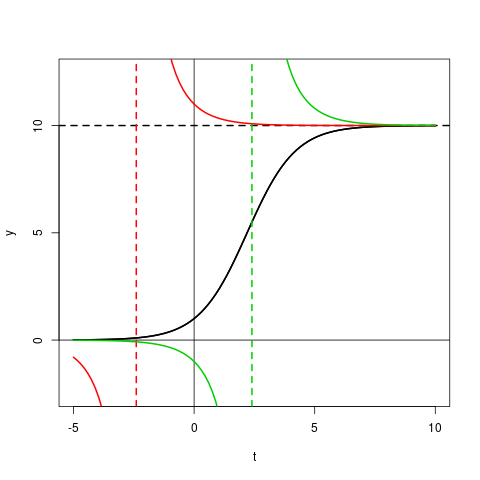
\includegraphics[width=.6\textwidth]{Verhulst-solutions}
  $$
  On remarque cependant que
  \begin{align*}
    y_0 & < 0 & \Rightarrow \quad |y_0| & < |K - y_0| & 
    \Rightarrow \quad |a_0| & < 1 & \Rightarrow \quad t_* & > 0, \\
    y_0 & > K & \Rightarrow \quad |y_0| & > |K - y_0| & 
    \Rightarrow \quad |a_0| & > 1 & \Rightarrow \quad t_* & < 0.
  \end{align*}
  On doit donc distinguer deux cas.
  \begin{itemize}
    \item $y(0) = y_0 > K$ (soit $t^* < 0$) : dans ce cas, on a toujours
    $$
    \lim_{t \to \infty} y(t) = K,
    $$
    et $y^* = K$ est un équilibre stable.
    \item $y(0) = y_0 < 0$ (soit $t^* > 0$) : la limite précédente reste vraie, mais, puisque
    $$
    \lim_{t \uparrow t^*} y(t) 
    = \lim_{t \uparrow -\log(-a_0) / r}  \frac{K a_0 e^{rt}}{1 +  a_0 e^{rt}}
    = -\infty,
    $$
    $y(t)$ atteint $- \infty$ en un temps fini $t^*$. $y^* = 0$ est donc un équilibre instable ($y^* = K$ est un équilibre stable, mais il ne sera jamais atteint).
  \end{itemize}
\end{description}

\remark
Le modèle de Verhulst est un des rares modèles non-linéaires pour lesquels il existe une solution explicite. Il n'est cependant pas nécessaire de disposer d'une solution explicite pour étudier la stabilité d'un équilibre.

\begin{theorem}[Stabilité ($n = 1$)]
  Pour $n=1$, un point d'équilibre $y^*$ est stable si $F'(y^*) < 0$ et instable si $F'(y^*) > 0$.
\end{theorem}

\proof Non démontré. \eproof

\remark
On obtient une intuition de ce résultat en étudiant la fonction $h(t) = y(t) - y^*$ au voisinage de $y(t) = y^*$. On a
$$
\dot h(t) = \dot y(t) = F(y(t)) = F(y^* + h(t)) = \underset{=0}{\underbrace{F(y^*)}} + F'(y^*) h(t) + o(\|h(t)\|),
$$
$h(t)$ se comporte donc localement comme la solution de 
$$
\dot h(t) = F'(y^*) h(t)
$$
soit $e ^{F'(y^*) t}$ qui tend vers 0 si $F'(y^*) < 0$ et vers l'infini si $F'(y^*) > 0$.

\exemple{
  Dans le cas du modèle de Verhulst, on a $F(y) = y(r - cy)$, soit
  $$
  F'(y) = r - 2cy
  $$
  qui est bien positive pour $y = 0$ (équilibre instable) et négative pour $y = K = r/c$ (équilibre stable).
}

%-------------------------------------------------------------------------------
\paragraph*{Notion de bifurcation.}
De nombreux systèmes dynamiques sont exprimés en fonction de paramètres dont dépendent les points d'équilibre et leur nature. Des valeurs proches des paramètres donnent des points d'équilibres proches et de même nature. La théorie des bifurcations s'intéresse aux régions de l'espace des paramètres au sein desquelles les points d'équilibres restent de même nature : plus précisément elle s'intéresse aux frontières entre ces régions.

%-------------------------------------------------------------------------------
\exemple{
  On étudie les points d'équilibre du système 
  $$
  \dot y = F(y) = \mu y - y^3
  $$
  et on souhaite déterminer leur nature. \\
  On a 
  $$
  F(x) = x(\mu - x^2) = 0 
  \qquad \Leftrightarrow \qquad
  x \in \left\{\begin{array}{ll} 
      \{-\sqrt{\mu}, 0, \sqrt{\mu}\} & \text{si } \mu > 0 \\
      \{0\} & \text{si } \mu \leq 0
    \end{array}\right.
  $$ 
  De plus, 
  $$
  F'(x) = \mu - 3 x^2
  $$
  donc
  \begin{itemize}
    \item si $\mu < 0$, $0$ le seul équilibre et il est stable, , 
    \item si $\mu > 0$, $0$ est instable mais $-\sqrt{\mu}$ et $\sqrt{\mu}$ sont stables. 
  \end{itemize}
  On peut ainsi tracer le {\em diagramme de bifurcation}.
  $$
%  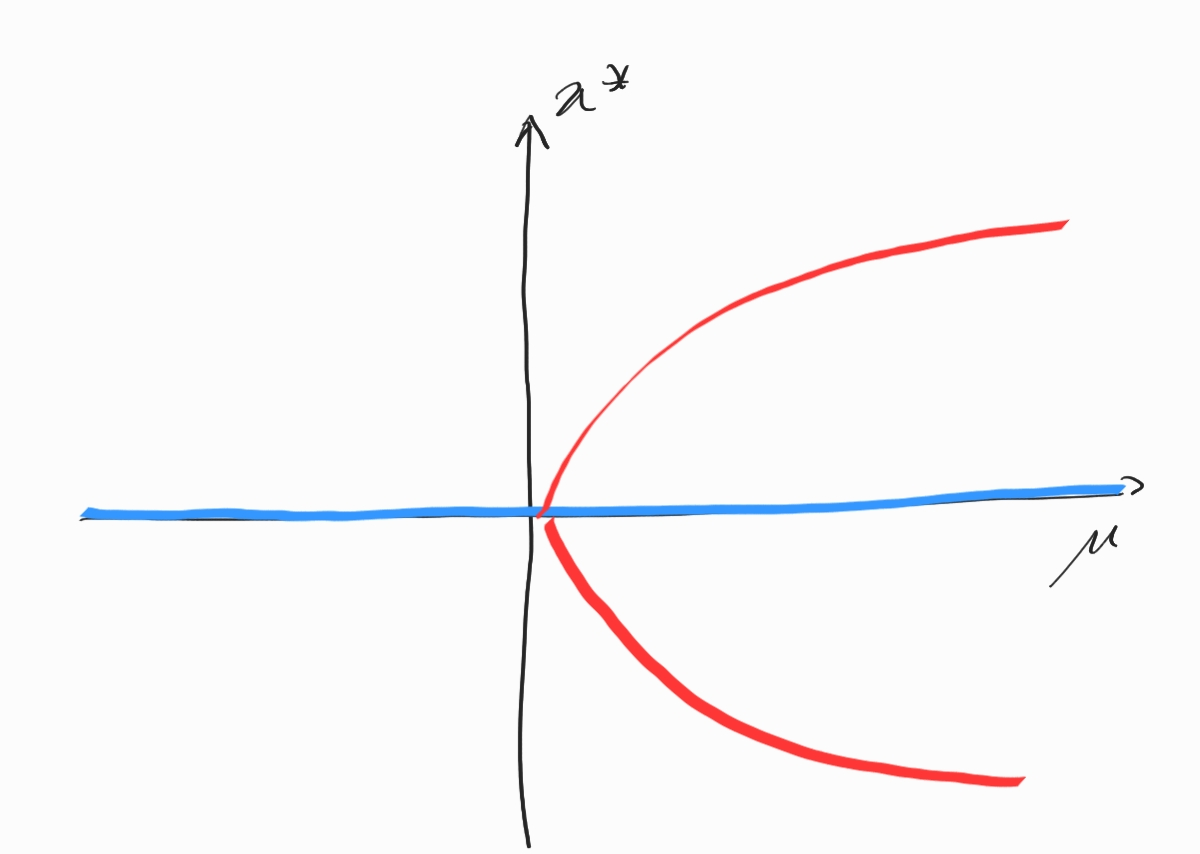
\includegraphics[width=.5\textwidth, trim=0 0 0 15, clip=]{StabiliteSystemeDynamique-Exemple1}
  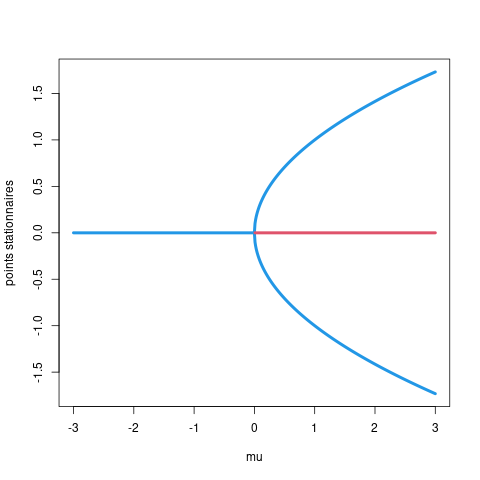
\includegraphics[width=.5\textwidth, trim=0 0 0 15, clip=]{StabiliteSystemeDynamique-Bifurcation}
  $$
}

% %-------------------------------------------------------------------------------
% \textcolor{gray}{
%   \exemple{
%     On souhaite déterminer les points d'équilibre (et leur nature) du système
%     $$
%     \dot y = F(y) = \mu y + 2 y^3 - y^5.
%     $$
%     On a 
%     $$
%     F(y) = y(\mu + y^2 - y^4)
%     $$
%     qui s'annule pour $y = 0$ et pour les solutions de $(\mu + 2 y^2 - y^4)$. En posant, $z = y^2$, $\mu + 2 z - z^2 = 0$ admet des solutions si $\Delta =  4(1 + \mu) \geq 0$, soit $\mu \geq -1$. Ces solutions sont alors $z^* = -1 \pm \sqrt{1+\mu}$. La seule solution possiblement positive est $z^* = -1 + \sqrt{1+\mu}$ et elle l'est ssi $\mu > 1$. \\
%     Le système admet donc un unique point fixe $y^*=0$ si $\mu < 1$ et un second point fixe $y^* = -1+\sqrt{1+\mu}$ si $\mu > 1$. \\
%     On a de plus
%     $$
%     F'(x) = \mu + 3 y^2 - 5y^4
%     $$
%     dont le signe est celui de $\mu$ pour $x=0$ et \todo{nature de $y^* = -1+\sqrt{1+\mu}$ si $\mu > 1$.}
%   }}

% %-------------------------------------------------------------------------------
% \exemple{[Exercice 2, TD2, L2 Bio SU]
%   On considère le système
%   $$
%   \dot y = - y^3 + 7 y^2 - 14 y + 8.
%   $$
%   Ses points stationnaires sont les racines du polynôme $P(y) = - y^3 + 7 y^2 - 14 y + 8$, donc $y_1 = 1$ fait partie, donc
%   $$
%   P(y) = (y-1) (-y^2 + 6y + 8),
%   $$
%   et les deux racines de $-y^2 + 6y + 8$ sont $2$ et $4$. Les points stationnaires du système sont donc 
%   $$
%   y_1 = 1, \qquad y_2 = 2, \qquad y_3 = 4.
%   $$
%   Leur stabilité est donné par la dérivée de $P$:
%   $$
%   P'(y) = -3y^2 + 14 y - 14,
%   $$
%   soit
%   $$
%   P'(y_1) = -3, \qquad P'(y_2) = 2, \qquad P'(y_3) = -6.
%   $$
%   $y_1$ et $y_3$ sont donc des équilibres stables, et $y_2$ un équilibre instable.
%   $$
%   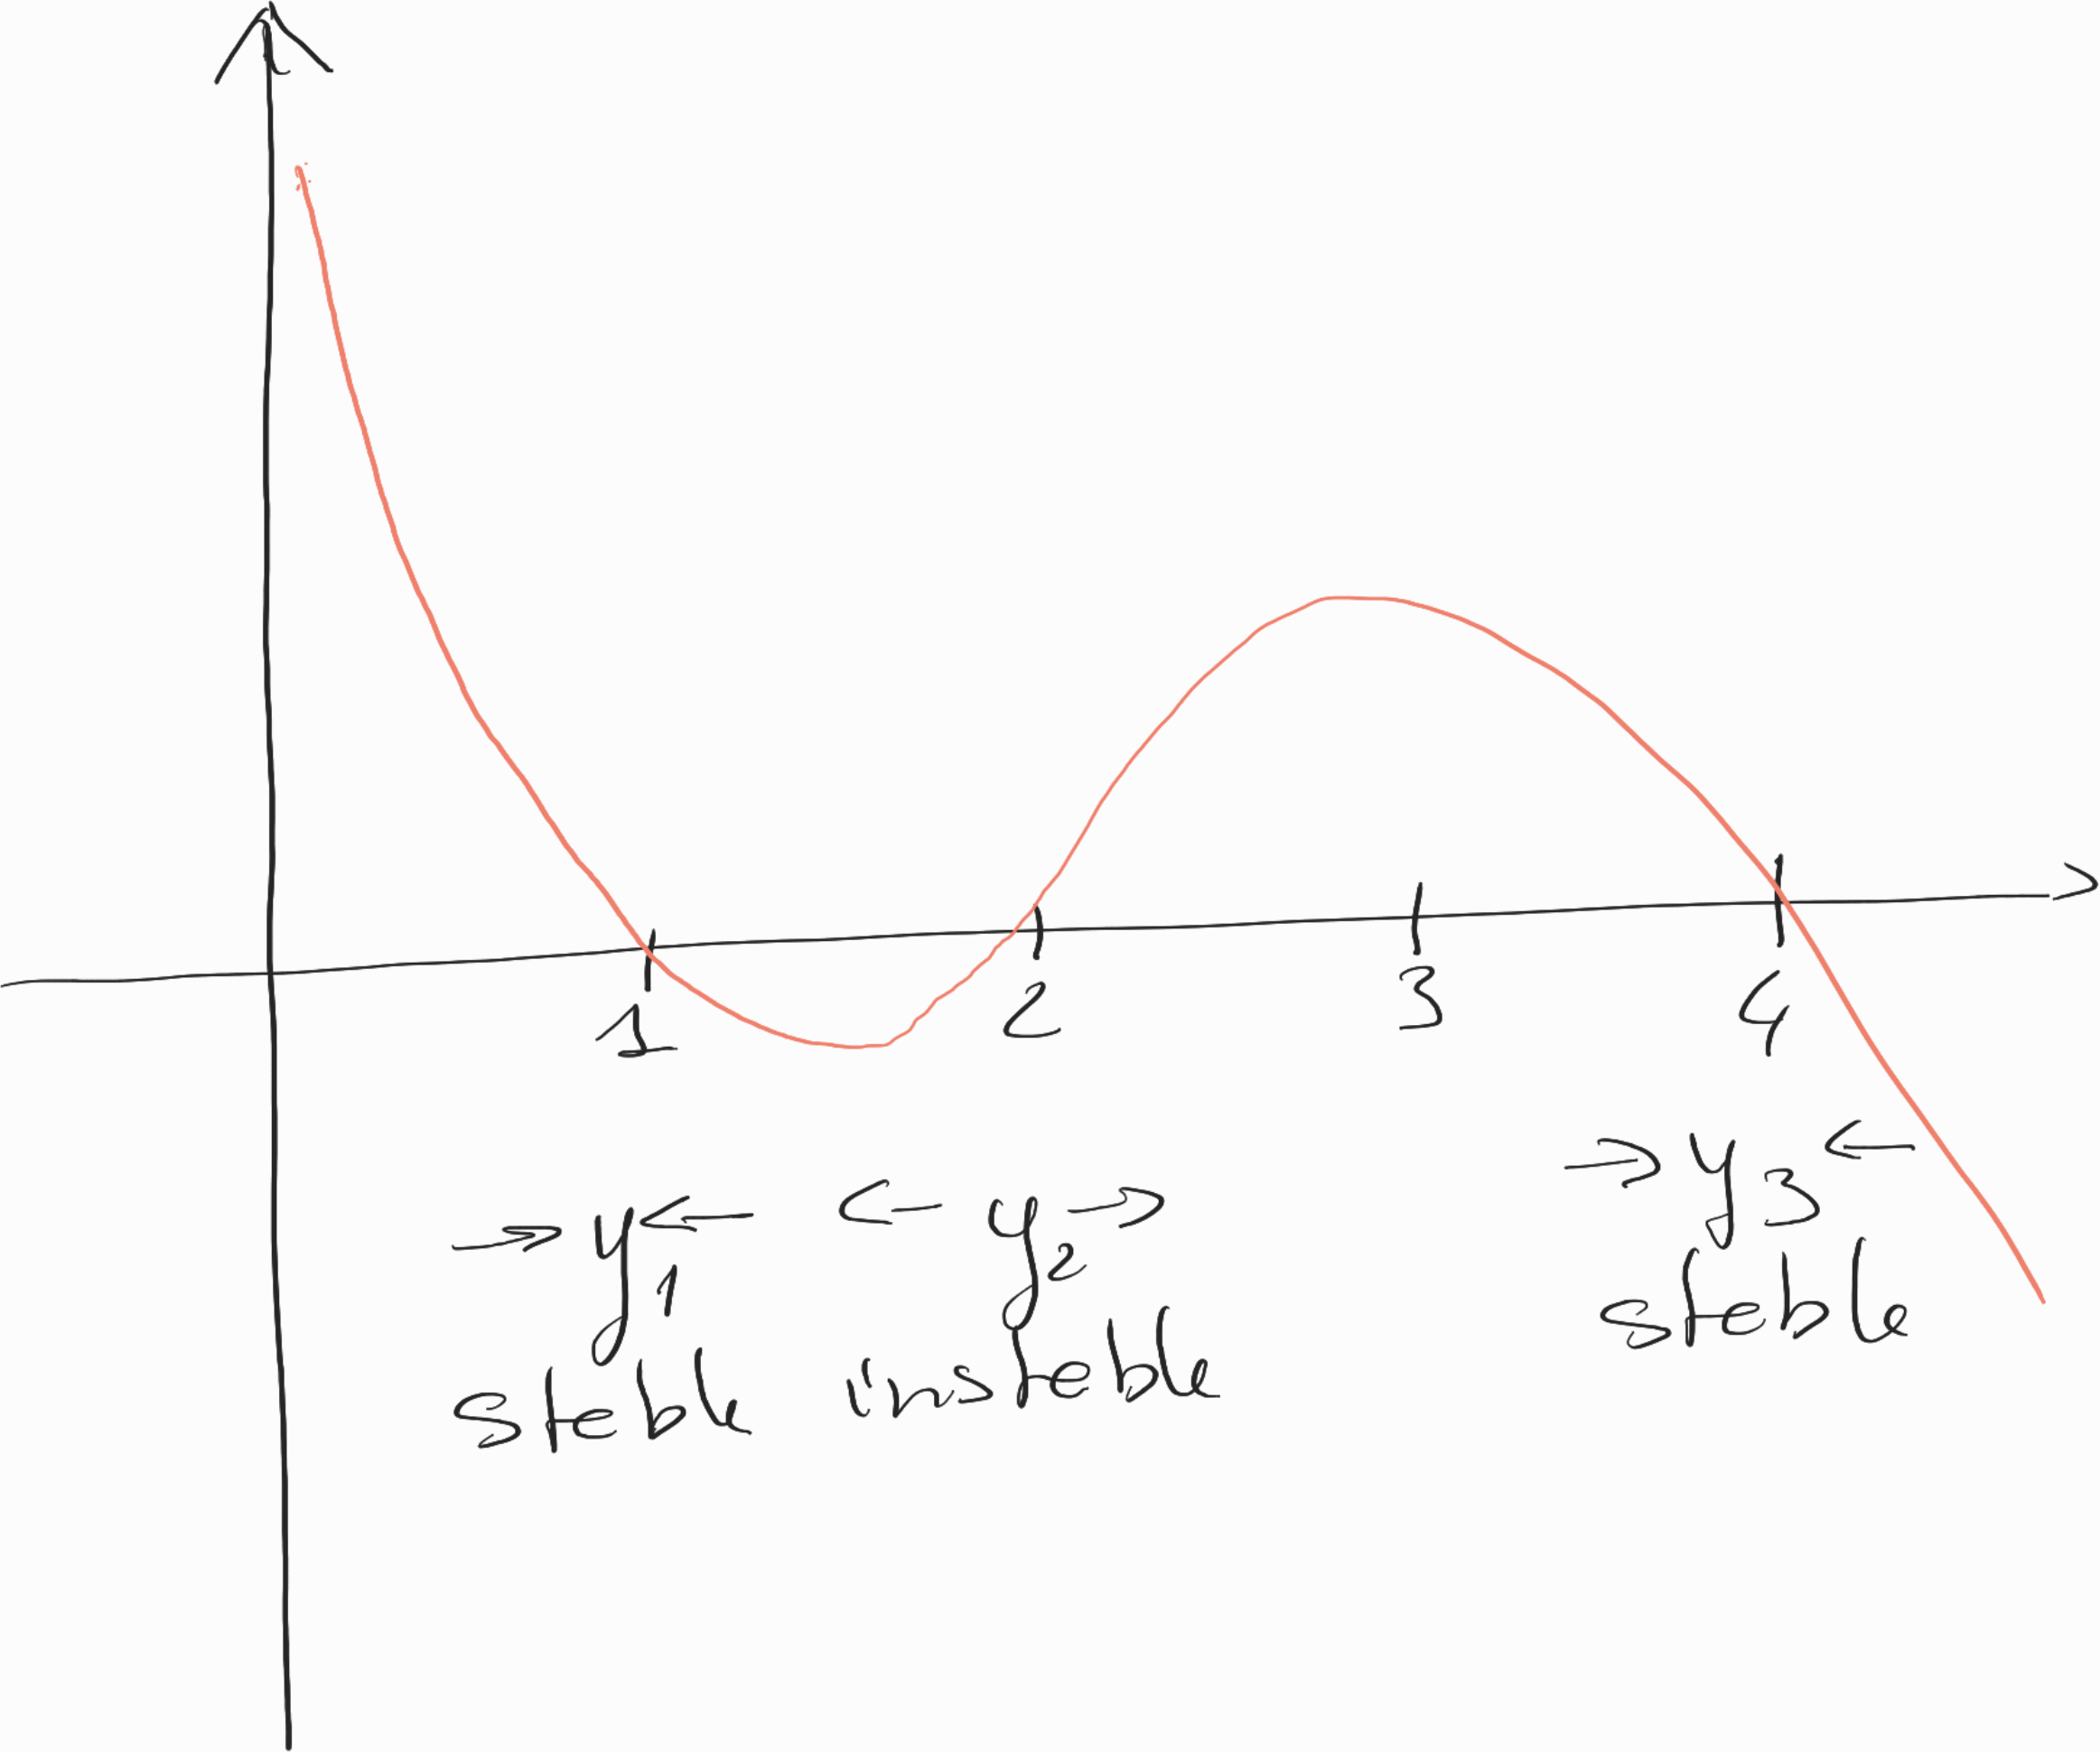
\includegraphics[width=.5\textwidth]{TD-SUbioL3-TD2Exo2}
%   $$
% }
